% !TeX spellcheck = de_DE
\newpage
\chapter{NetSimile}

\subsubsection{Eindimensionales Signal}
\label{sec:appendix_net_original}
\begin{figure}[H]
	\centering
	\subfloat[Ausrei�ertyp Signal Drift\label{img:dailyDriftNetOne}]{
		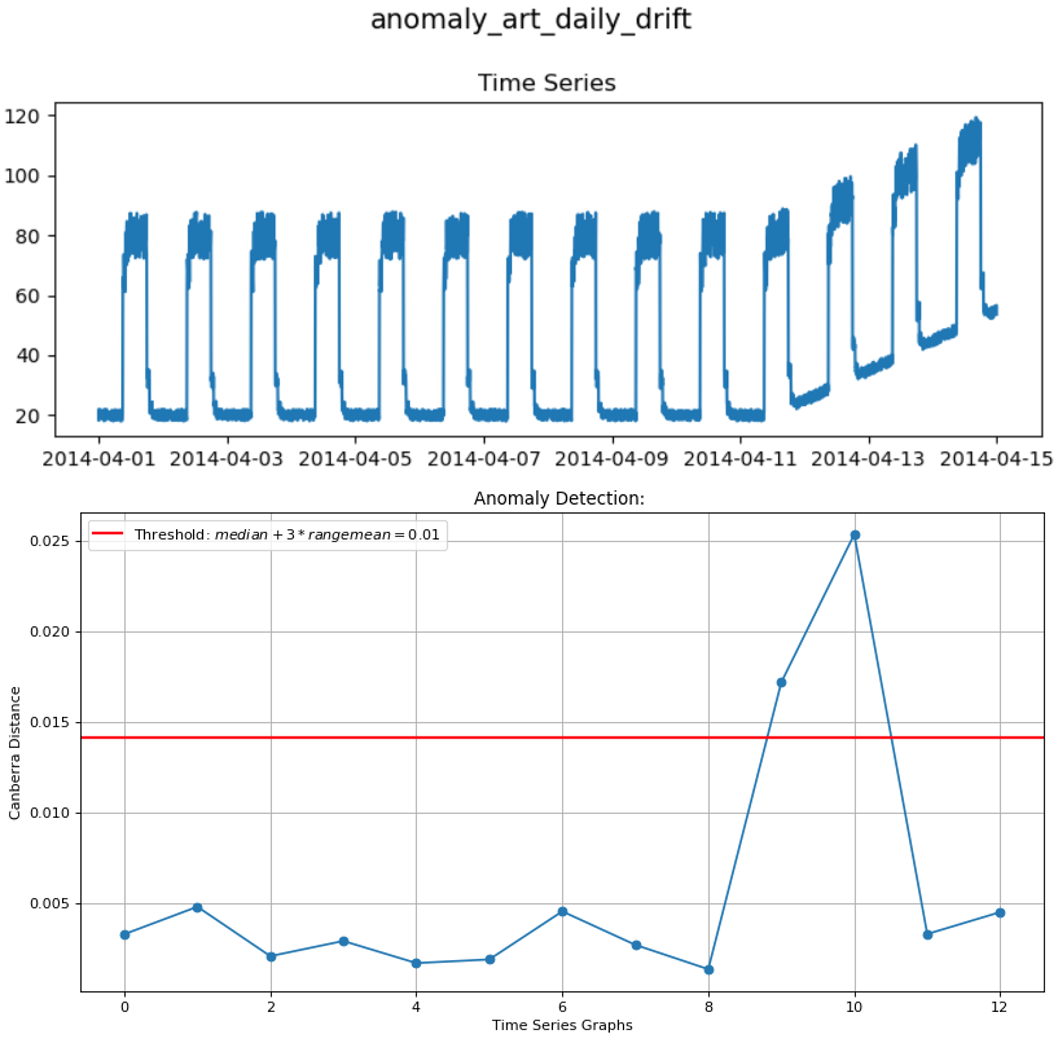
\includegraphics[width=0.5\textwidth]{fig/resultsNetismile/original/daily_drift}}
	\subfloat[Ausrei�ertyp Zunahme am Rauschen\label{img:increaseNoiseNetOne}]{
		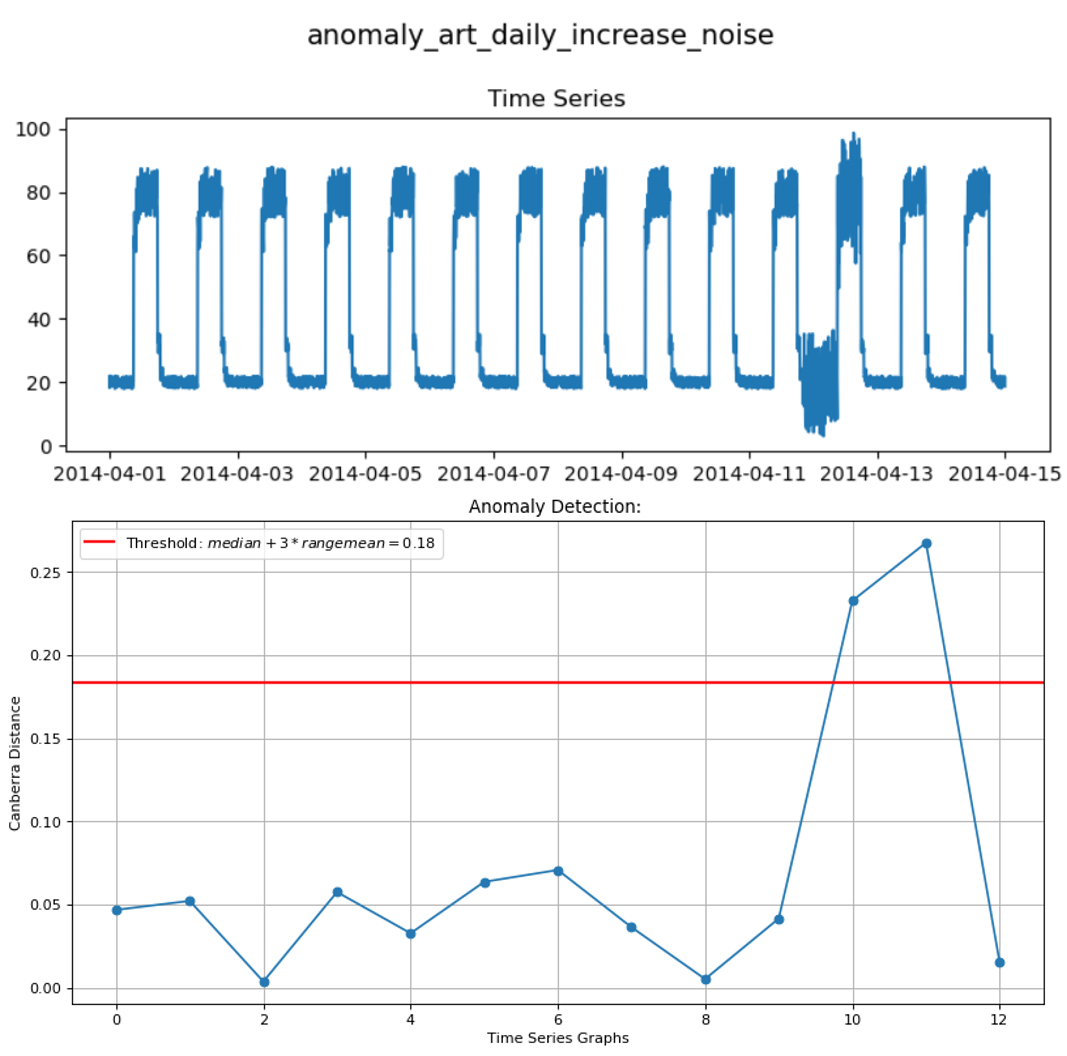
\includegraphics[width=0.5\textwidth]{fig/resultsNetismile/original/increase_noise}}
	\qquad
	\subfloat[Ausrei�ertyp Einzelne Peaks\label{img:dailyPeaksNetOne}]{
		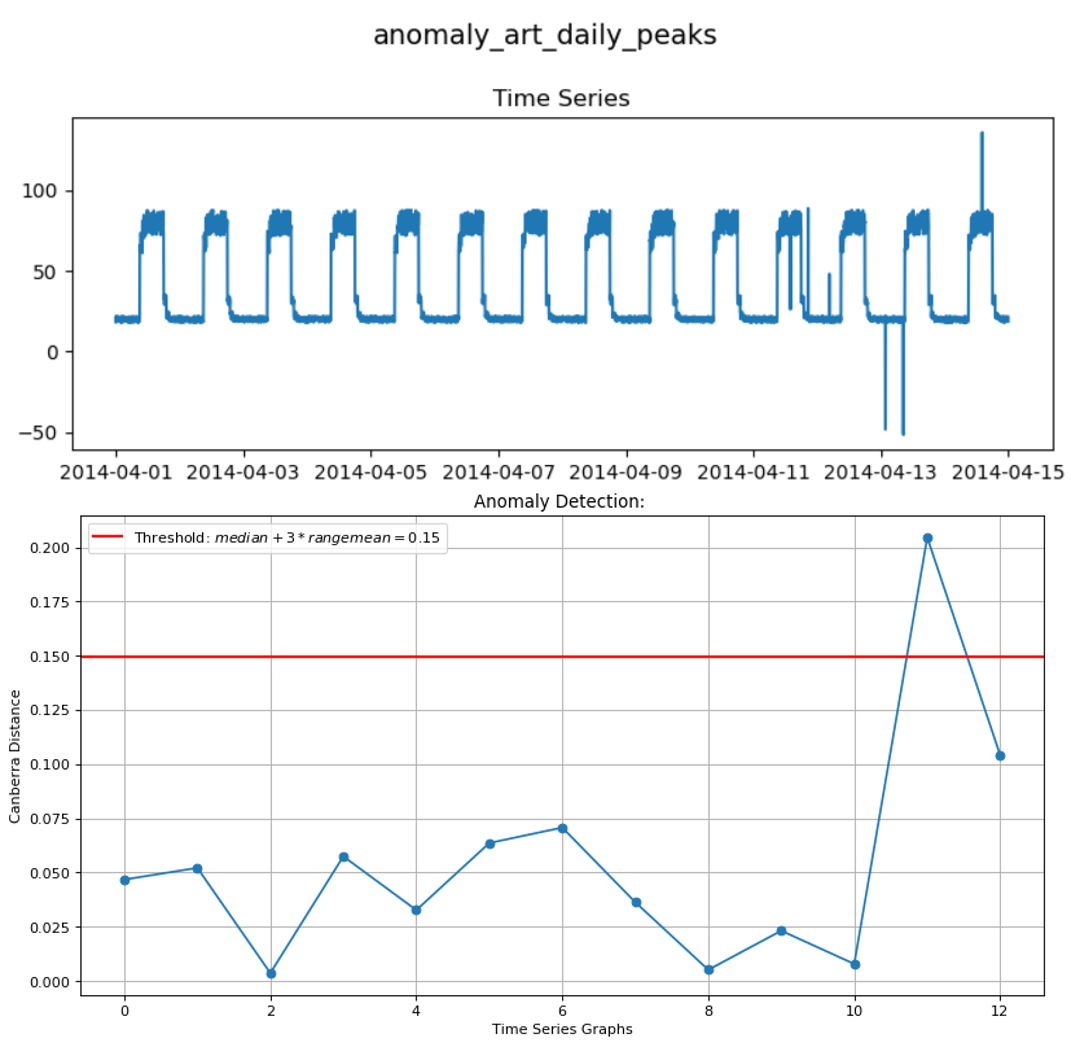
\includegraphics[width=0.5\textwidth]{fig/resultsNetismile/original/daily_peaks}}
	\subfloat[Ausrei�ertyp Frequenz�nderung\label{img:sequenceChangeNetONe}]{		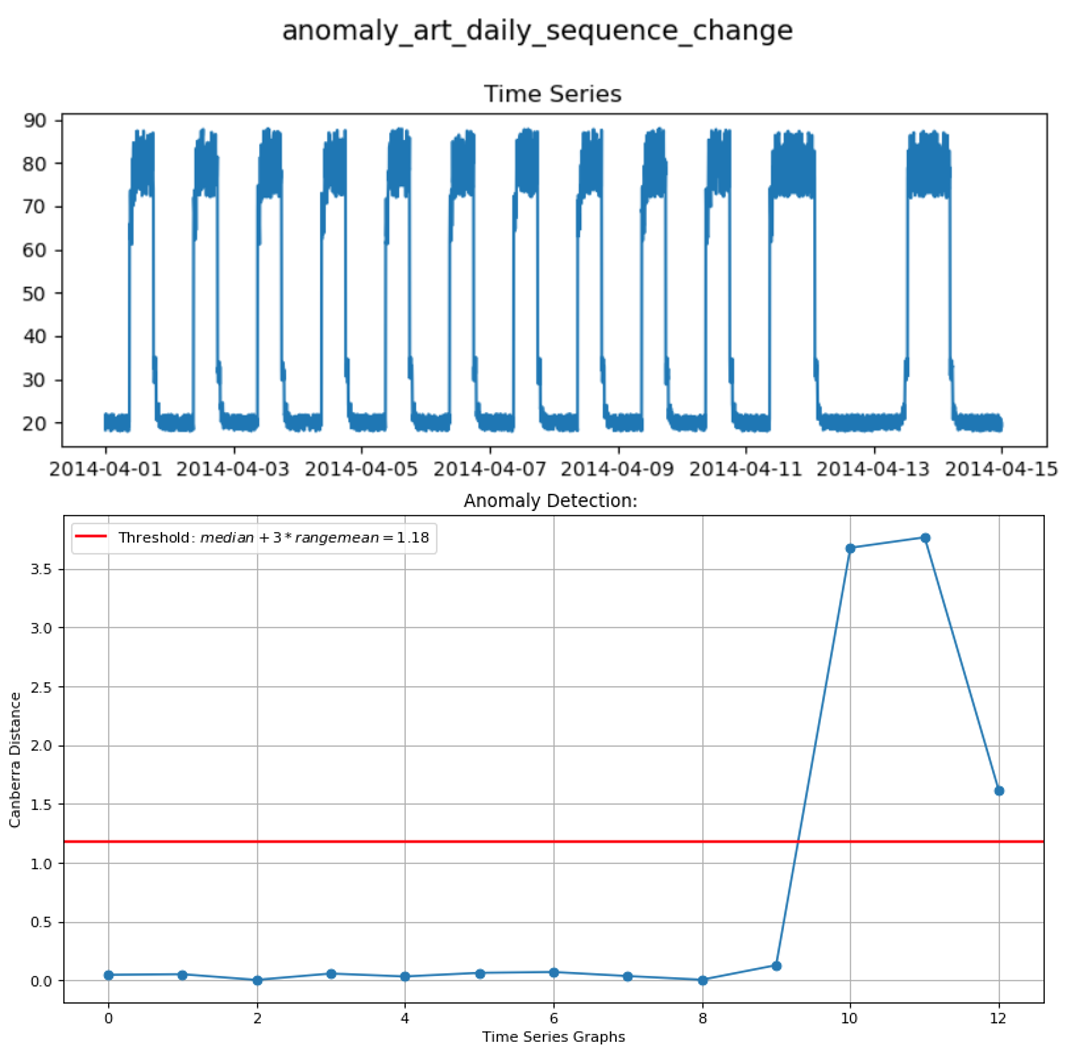
\includegraphics[width=0.5\textwidth]{fig/resultsNetismile/original/sequence_change}}
	\qquad
\end{figure}
\begin{figure}\ContinuedFloat
	\subfloat[Ausrei�ertyp Kontinuierliche Zunahme der Amplitude\label{img:ampRiseNetOne}]{
		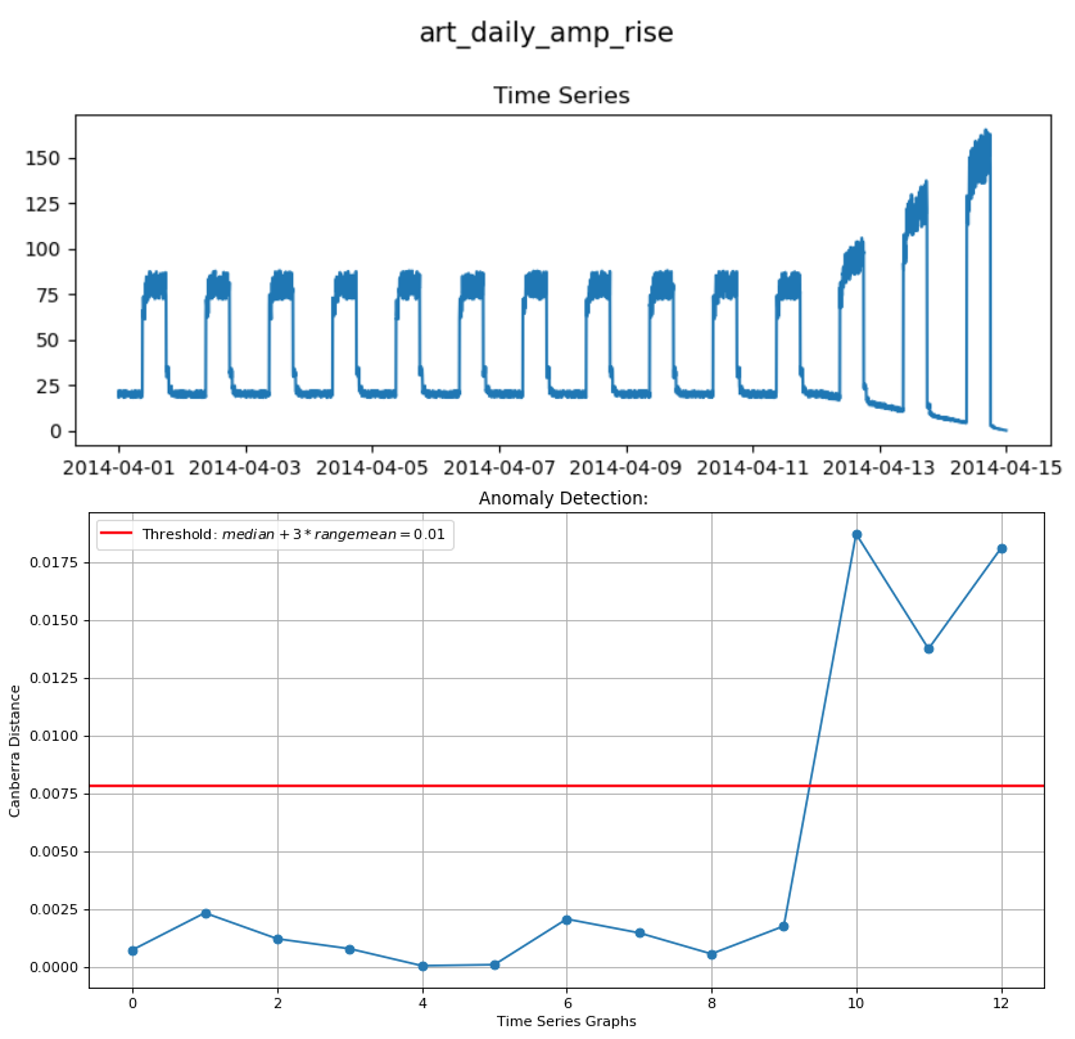
\includegraphics[width=0.5\textwidth]{fig/resultsNetismile/original/amp_rise}}
	\subfloat[Ausrei�ertyp Zyklus Aussetzer\label{img:flatmiddleNetOne}]{
		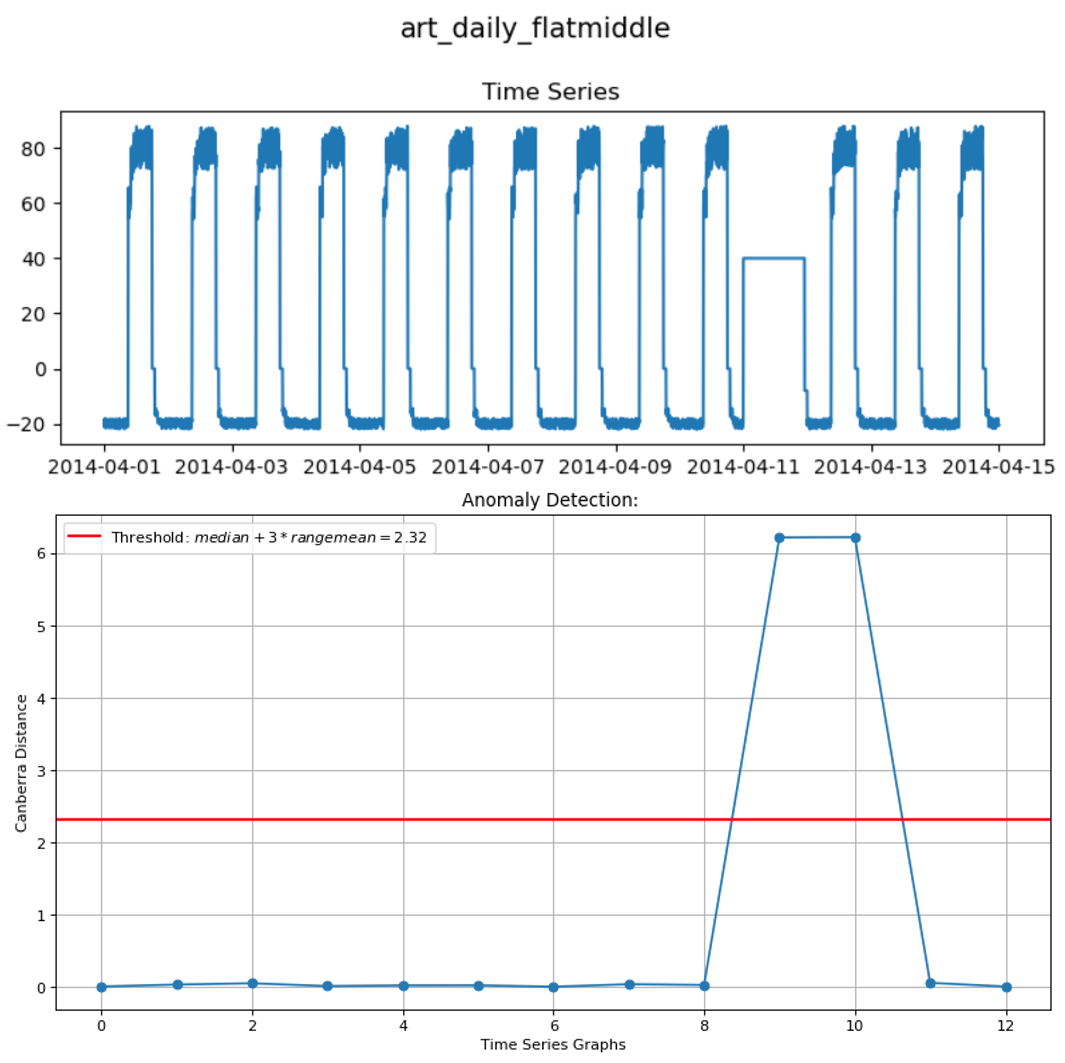
\includegraphics[width=0.5\textwidth]{fig/resultsNetismile/original/flatmiddle}}
	\qquad
	\subfloat[Ausrei�ertyp Zyklus mit geringerer Amplitude\label{img:jumpsdownNetOne}]{
		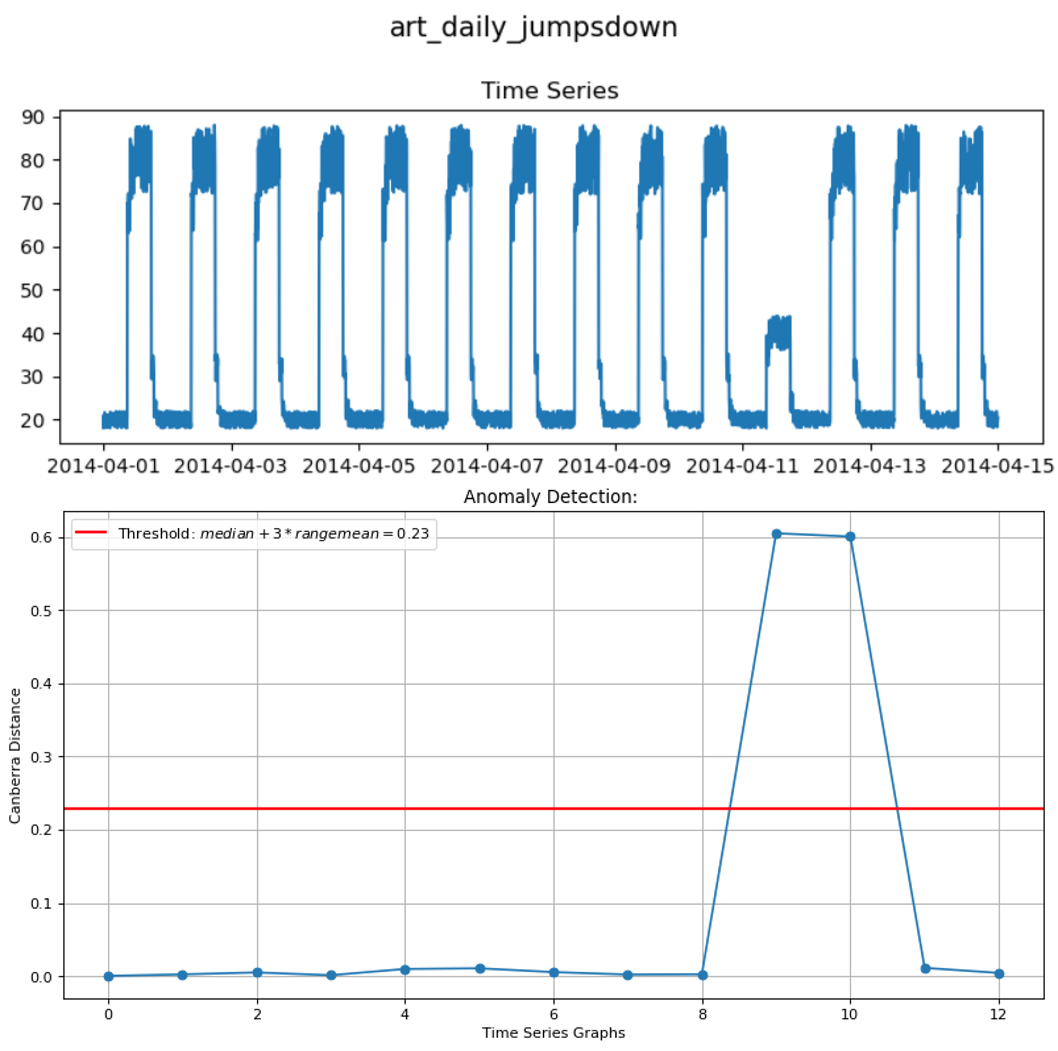
\includegraphics[width=0.5\textwidth]{fig/resultsNetismile/original/jumpsdown}}
	\subfloat[Ausrei�ertyp Zyklus mit h�herer Amplitude\label{img:jumpsupNetOne}]{
		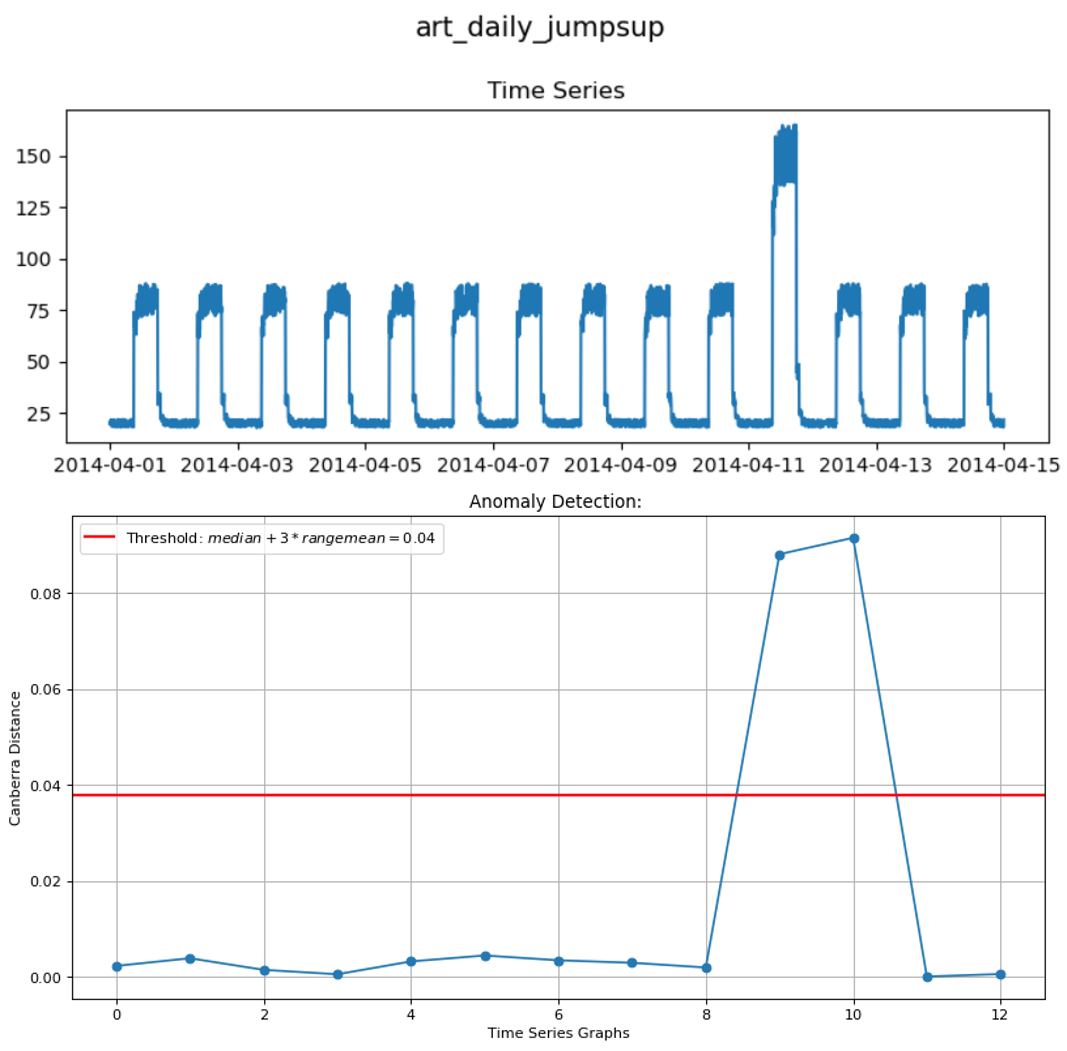
\includegraphics[width=0.5\textwidth]{fig/resultsNetismile/original/jumpsup}}
	\qquad
\end{figure}
\begin{figure}\ContinuedFloat
	\subfloat[Ausrei�ertyp Signal-Aussetzer\label{img:nojumpNetOne}]{
		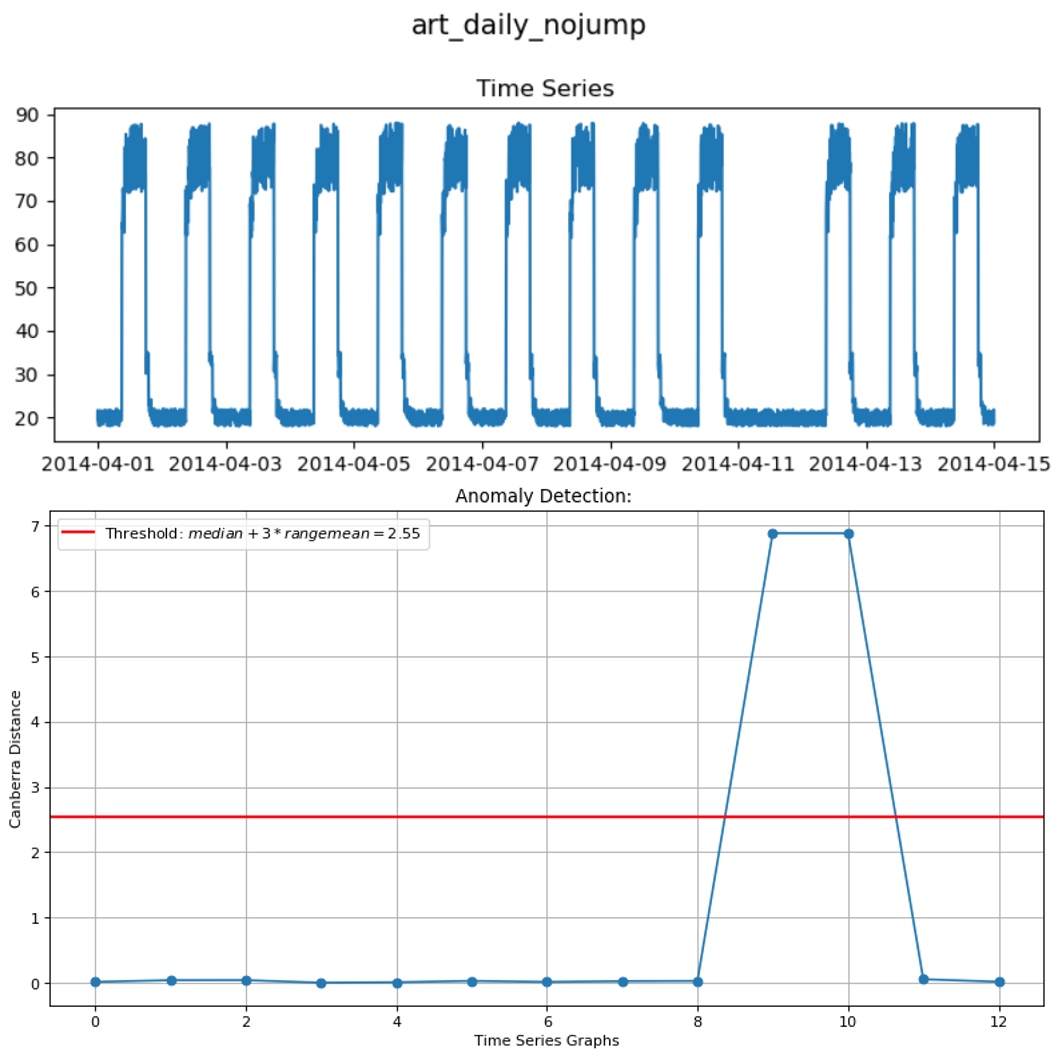
\includegraphics[width=0.5\textwidth]{fig/resultsNetismile/original/nojump}}
	\qquad
\end{figure}

%\subsubsection{Eindimensionales Signal Optimierte Version}
%\label{sec:appendix_net_one}
%\begin{figure}[H]
%	\centering
%	\subfloat[Caption for sub-figure1]{
%		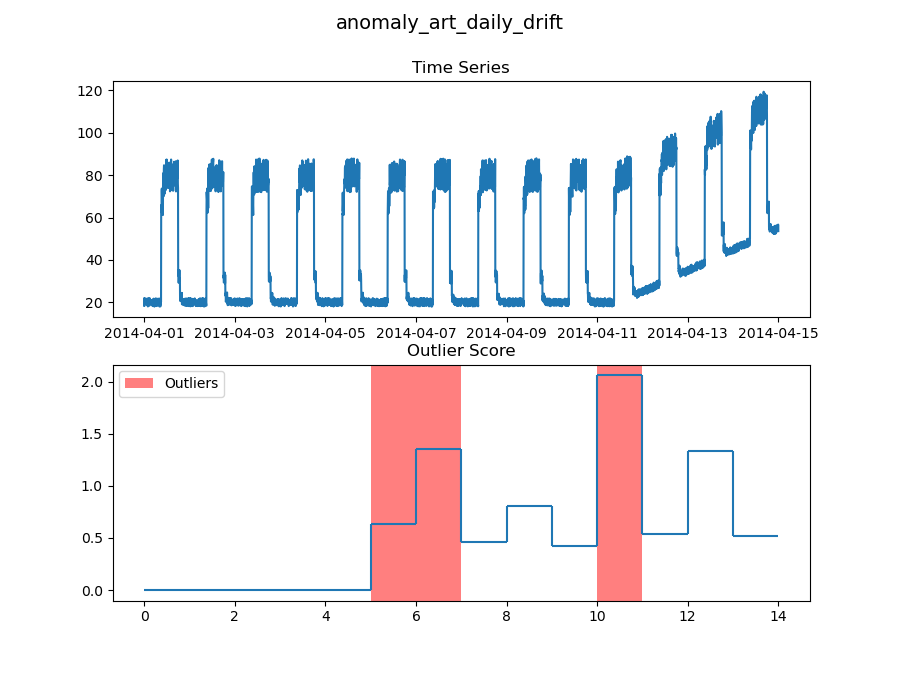
\includegraphics[width=0.5\textwidth]{fig/resultsNetismile/1D/anomaly_art_daily_drift}}
%	\subfloat[Caption for sub-figure1]{
%		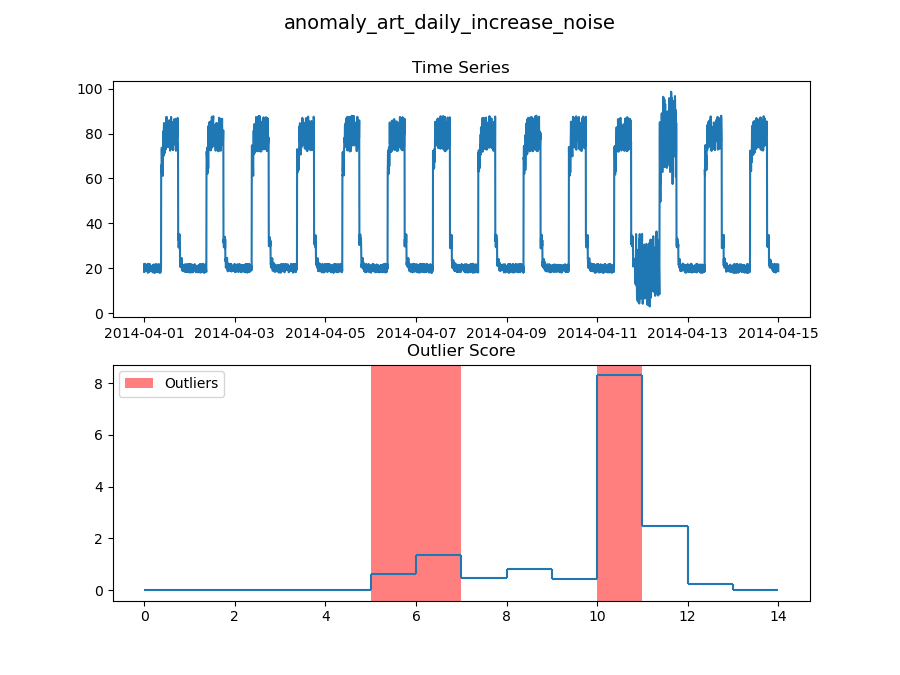
\includegraphics[width=0.5\textwidth]{fig/resultsNetismile/1D/anomaly_art_daily_increase_noise}}
%	\qquad
%	\subfloat[Caption for sub-figure1]{
%		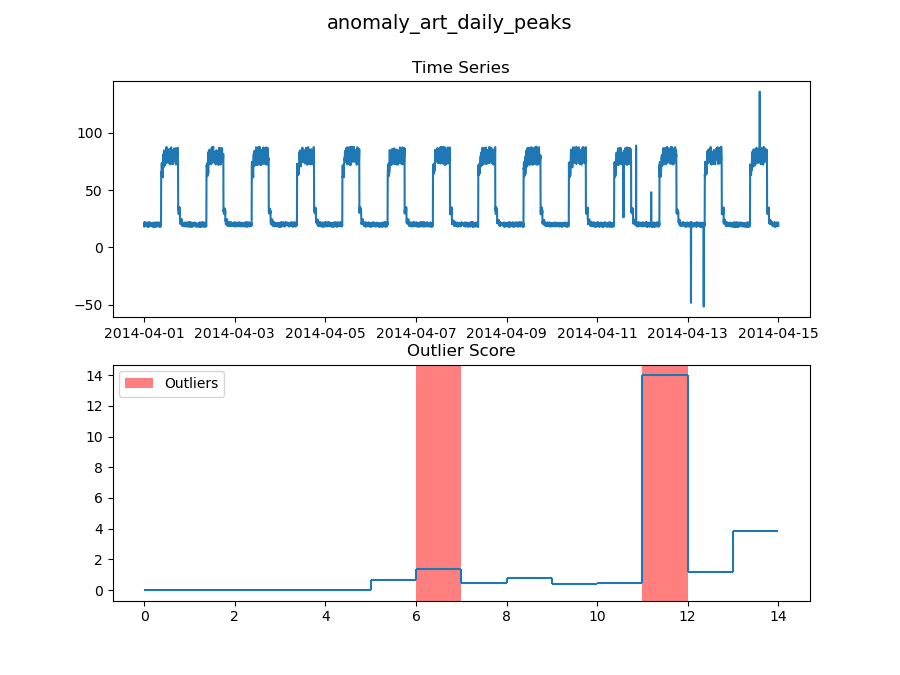
\includegraphics[width=0.5\textwidth]{fig/resultsNetismile/1D/anomaly_art_daily_peaks}}
%	\subfloat[Caption for sub-figure1]{
%		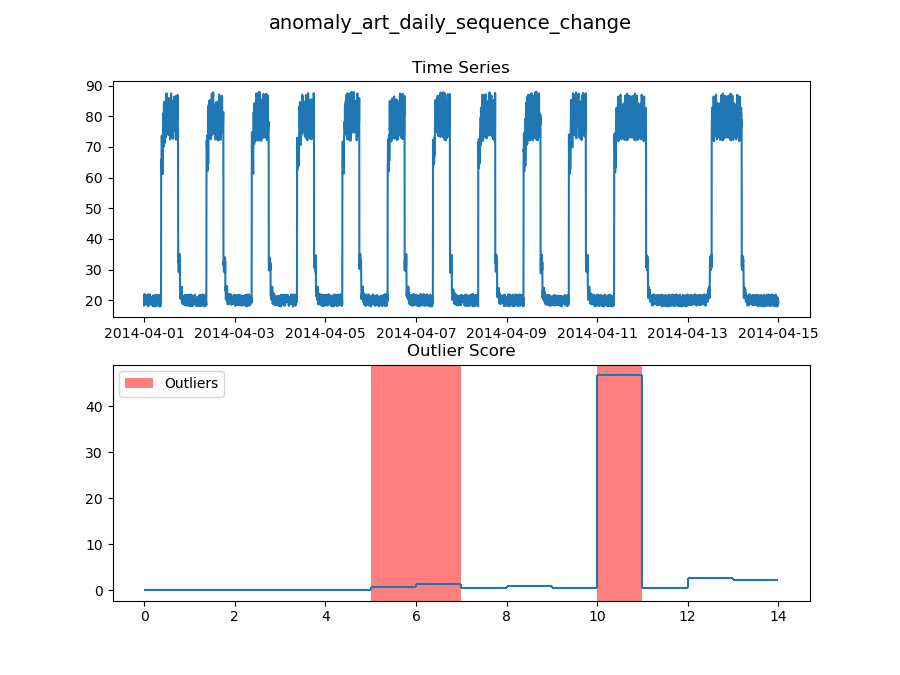
\includegraphics[width=0.5\textwidth]{fig/resultsNetismile/1D/anomaly_art_daily_sequece_change}}
%	\qquad
%	\label{img:isomappictures1}
%\end{figure}
%\begin{figure}\ContinuedFloat
%	\subfloat[Caption for sub-figure1]{
%		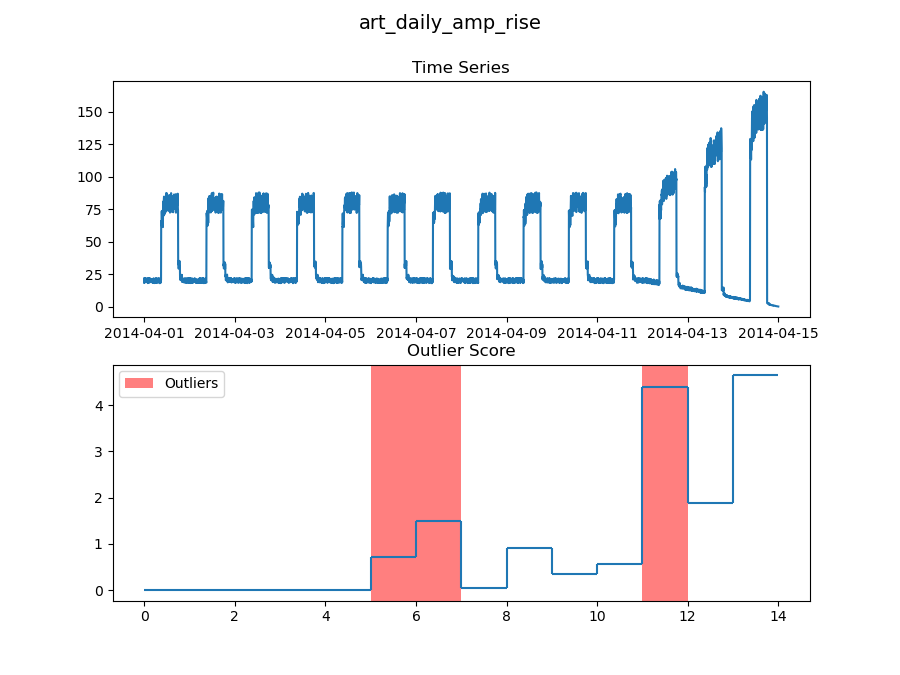
\includegraphics[width=0.5\textwidth]{fig/resultsNetismile/1D/art_daily_amp_rise}}
%	\subfloat[Caption for sub-figure1]{
%		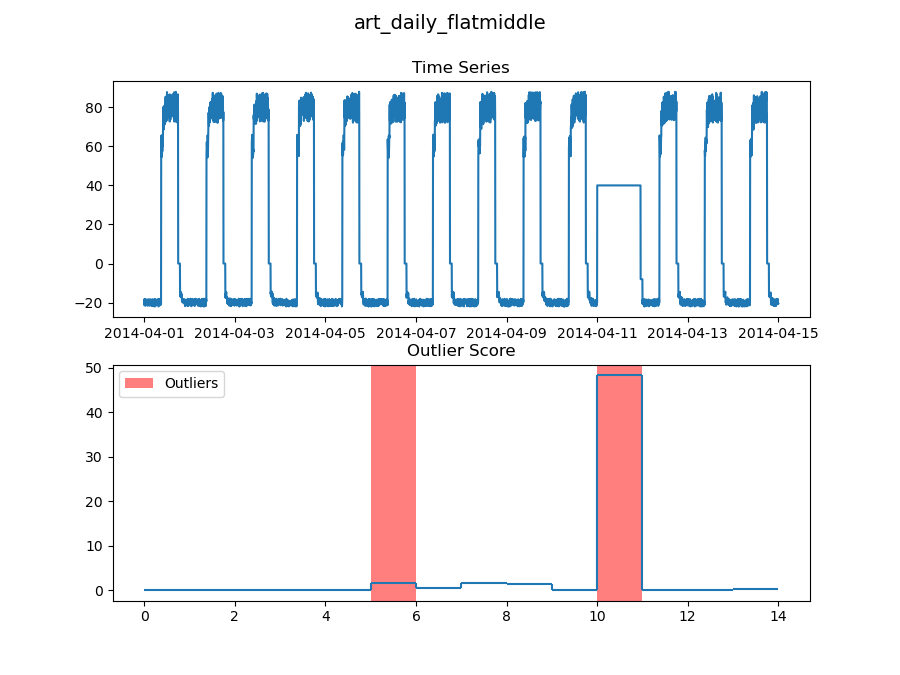
\includegraphics[width=0.5\textwidth]{fig/resultsNetismile/1D/art_daily_flatmiddle}}
%	\qquad
%	\subfloat[Caption for sub-figure1]{
%		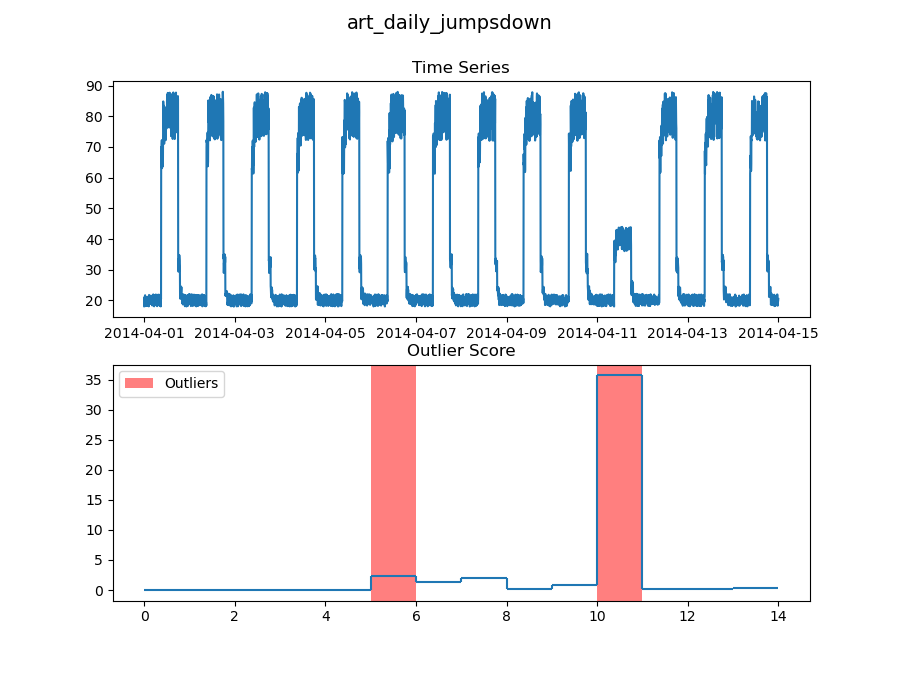
\includegraphics[width=0.5\textwidth]{fig/resultsNetismile/1D/art_daily_jumpsdown}}
%	\subfloat[Caption for sub-figure1]{
%		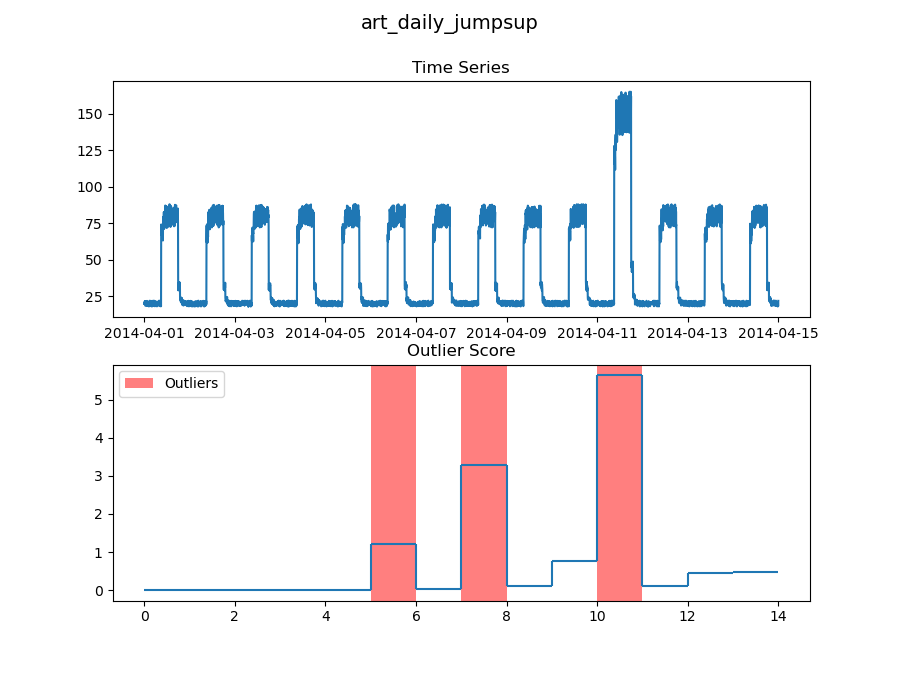
\includegraphics[width=0.5\textwidth]{fig/resultsNetismile/1D/art_daily_jumpsup}}
%	\qquad
%	\subfloat[Caption for sub-figure1]{
%		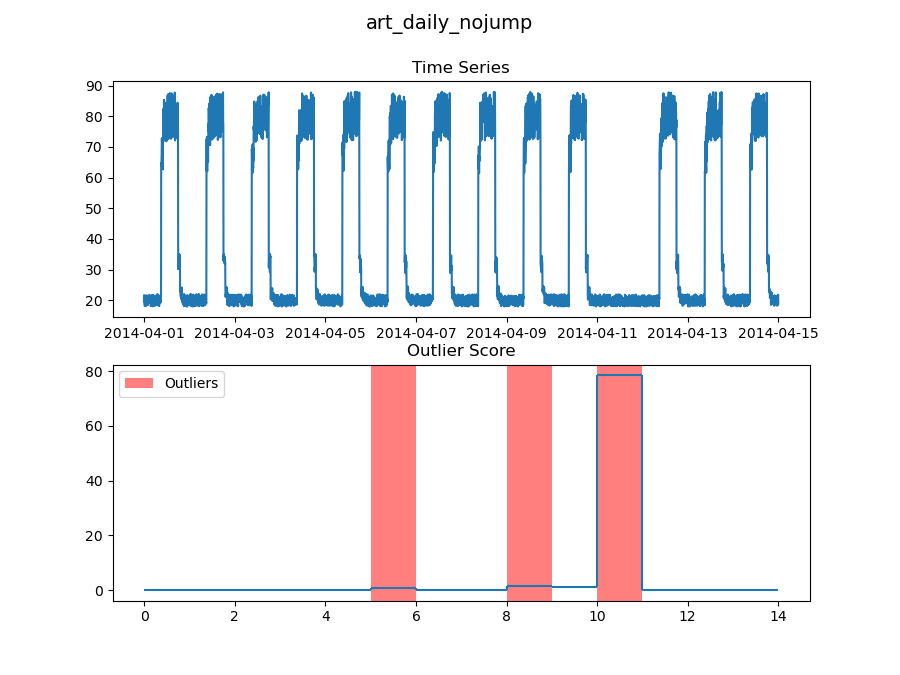
\includegraphics[width=0.5\textwidth]{fig/resultsNetismile/1D/art_daily_nojump}}
%	\label{img:isomappictures2}
%\end{figure}

%\workTodo{Wrong picture for daily peaks. Change that the sixed element is not always an outlier}

\newpage
\subsubsection{Zweidimensionales Signal}
\label{sec:appendix_net_two}
\begin{figure}[H]
	\centering
	\subfloat[Ausrei�er-Typ Signal Drift\label{img:dailyDriftNetTwo}]{
		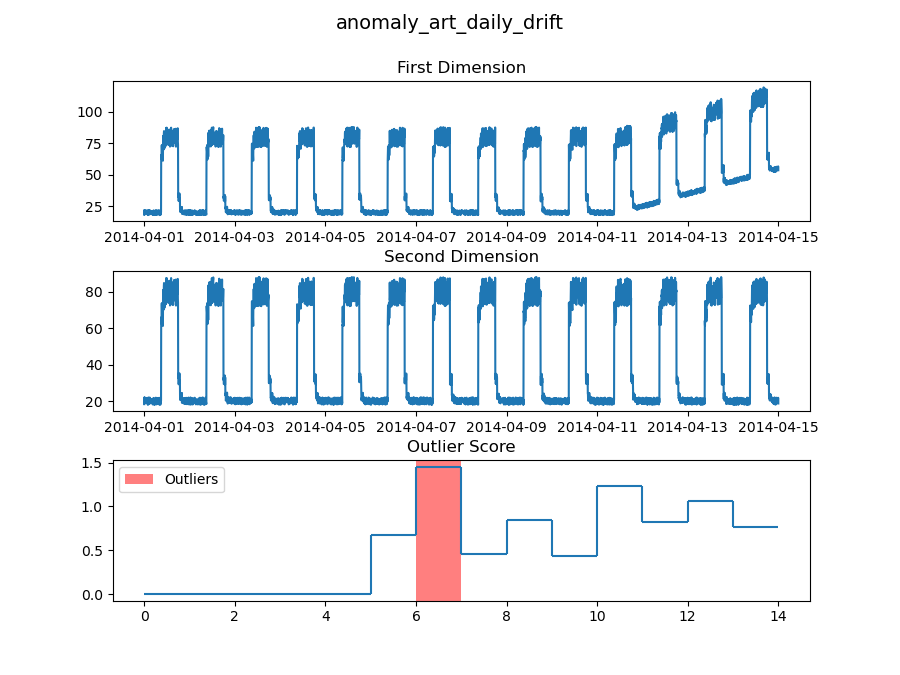
\includegraphics[width=0.5\textwidth]{fig/resultsNetismile/2D/anomaly_art_daily_drift}}
	\subfloat[Ausrei�er-Typ Zunahme an Rauschen\label{img:increaseNoiseNetTwo}]{
		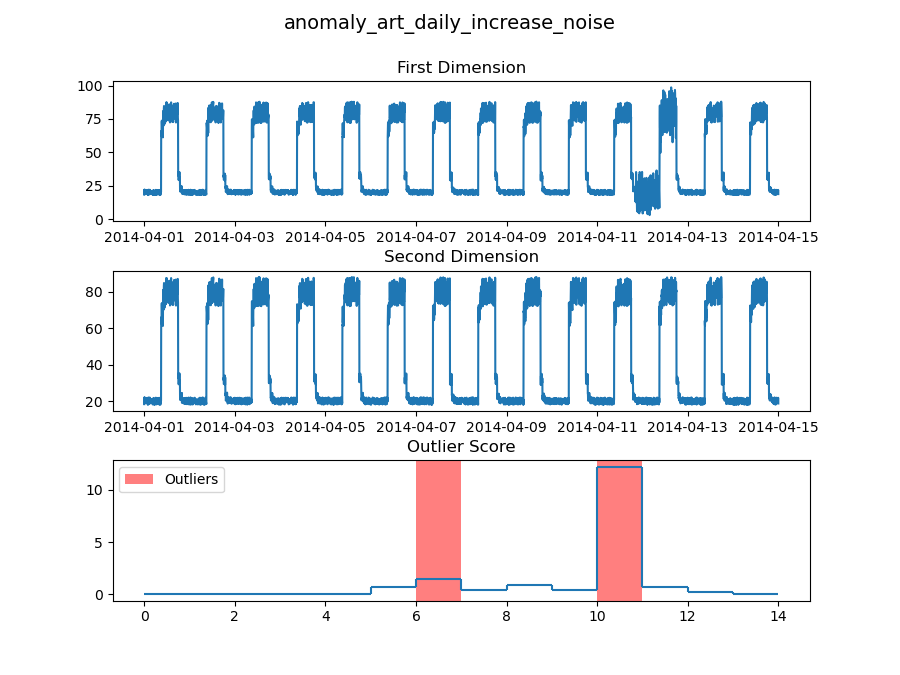
\includegraphics[width=0.5\textwidth]{fig/resultsNetismile/2D/anomaly_art_daily_increase_noise}}
	\qquad
	\subfloat[Ausrei�er-Typ Einzelne Peaks\label{img:dailyPeaksNetTwo}]{
		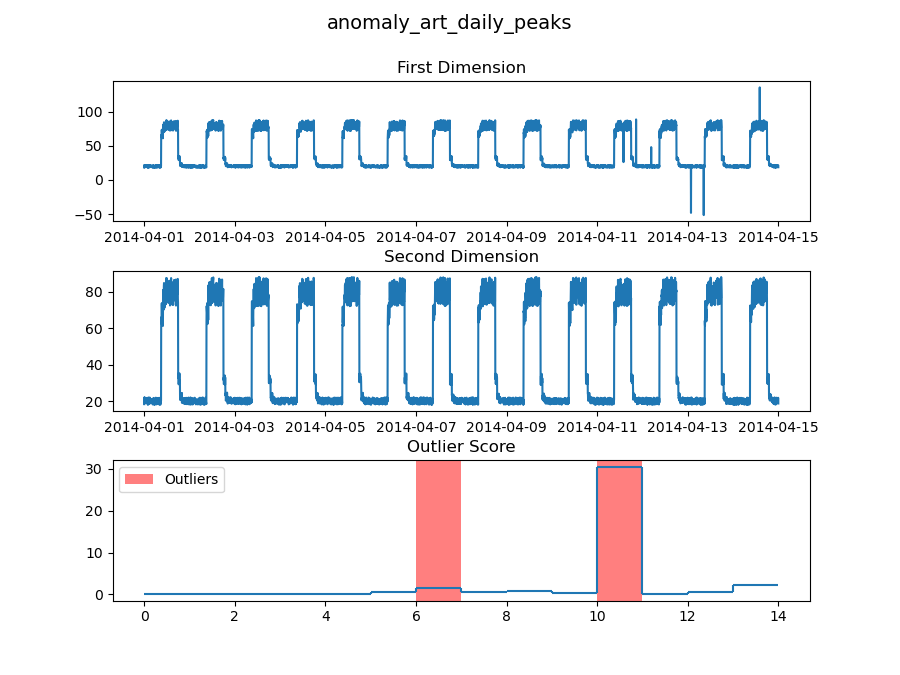
\includegraphics[width=0.5\textwidth]{fig/resultsNetismile/2D/anomaly_art_daily_peaks}}
	\subfloat[Ausrei�er-Typ Frequenz�nderung\label{img:sequenceChangeNetTwo}]{
		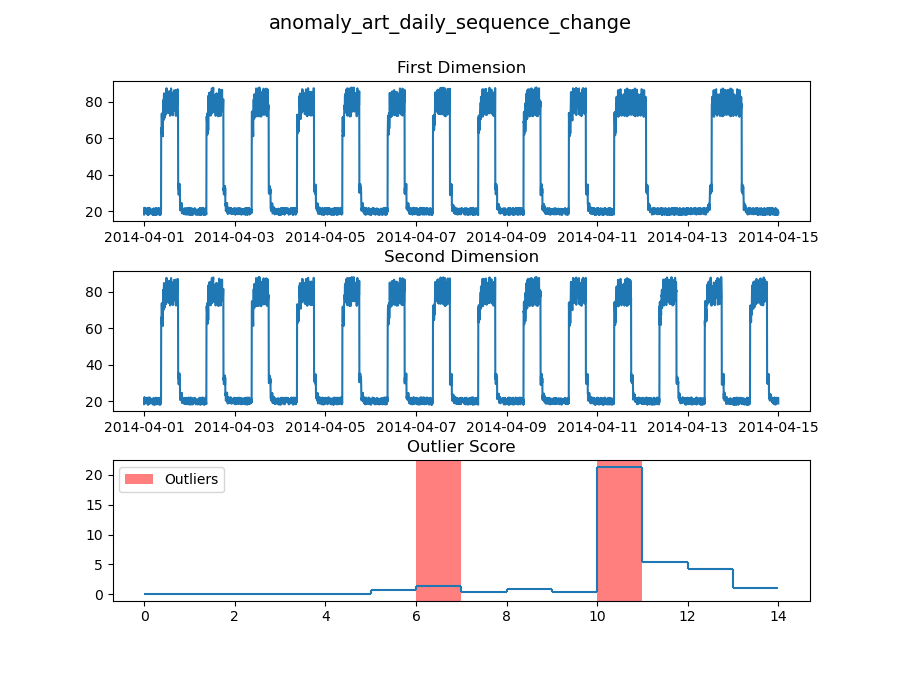
\includegraphics[width=0.5\textwidth]{fig/resultsNetismile/2D/anomaly_art_daily_sequence_change}}
	\qquad
	\label{img:isomappictures1}
\end{figure}
\begin{figure}\ContinuedFloat
	\subfloat[Ausrei�er-Typ Kontinuierliche Zunahme der Amplitude\label{img:ampRiseNetTwo}]{
		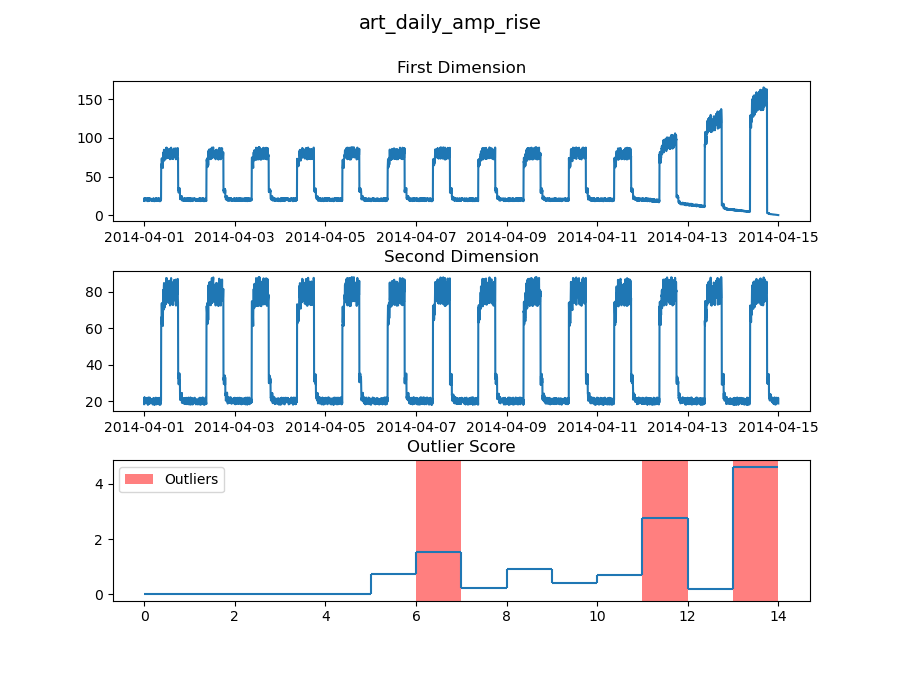
\includegraphics[width=0.5\textwidth]{fig/resultsNetismile/2D/art_daily_amp_rise}}
	\subfloat[Ausrei�er-Typ Zyklus-Aussetzer\label{img:flatmiddleNetTwo}]{
		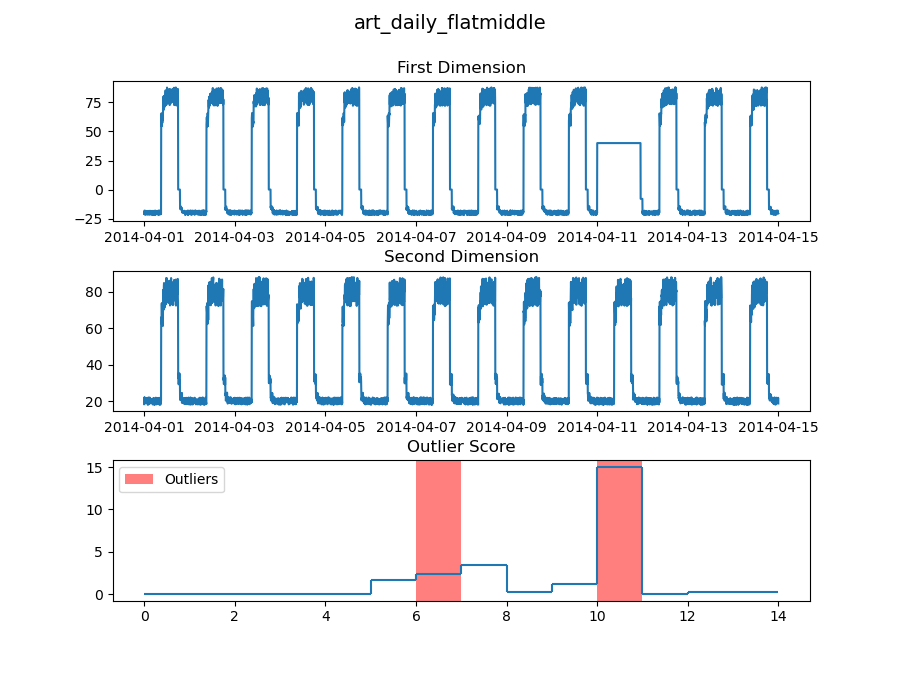
\includegraphics[width=0.5\textwidth]{fig/resultsNetismile/2D/art_daily_flatmiddle}}
	\qquad
	\subfloat[Ausrei�er-Typ Zyklus mit geringerer Amplitude\label{img:jumpsdownNetTwo}]{
		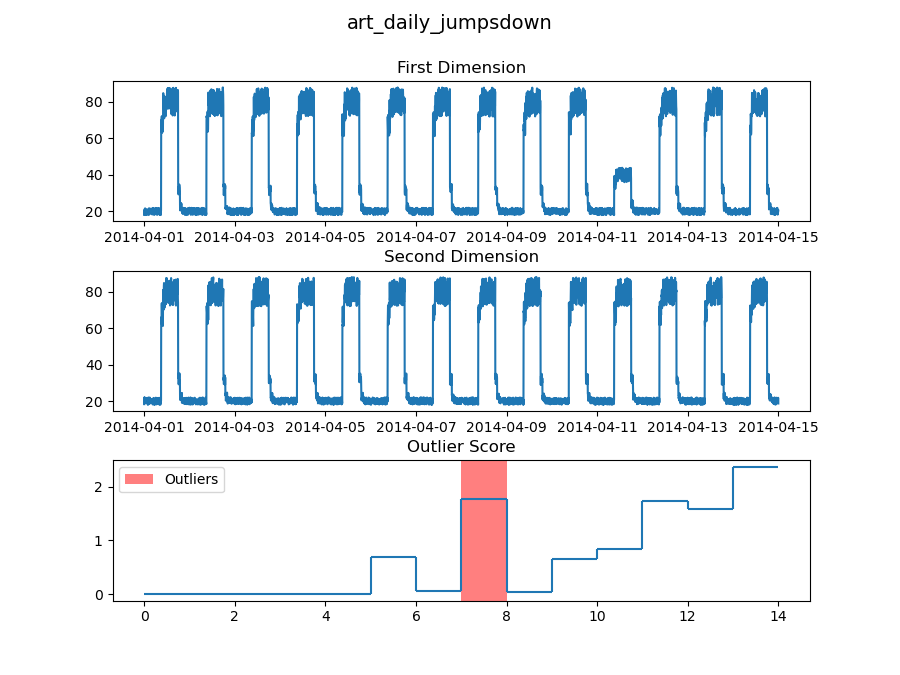
\includegraphics[width=0.5\textwidth]{fig/resultsNetismile/2D/art_daily_jumpsdown}}
	\subfloat[Ausrei�er-Typ Zyklus mit h�herer Amplitude\label{img:jumpsupNetTwo}]{
		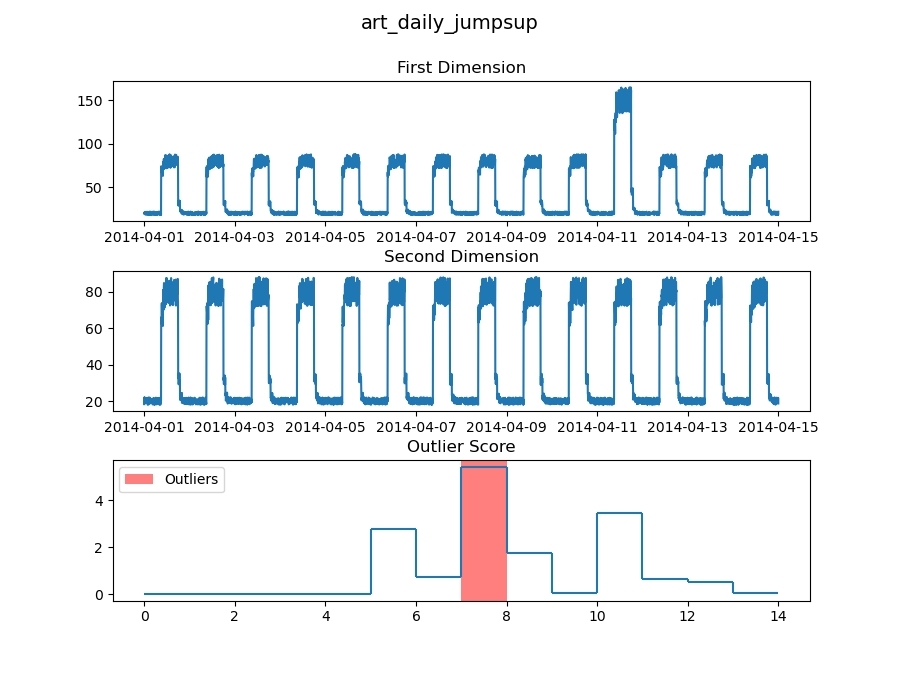
\includegraphics[width=0.5\textwidth]{fig/resultsNetismile/2D/art_daily_jumpsup}}
	\qquad
	\subfloat[Ausrei�er-Typ Signal-Aussetzer\label{img:nojumpNetTwo}]{
		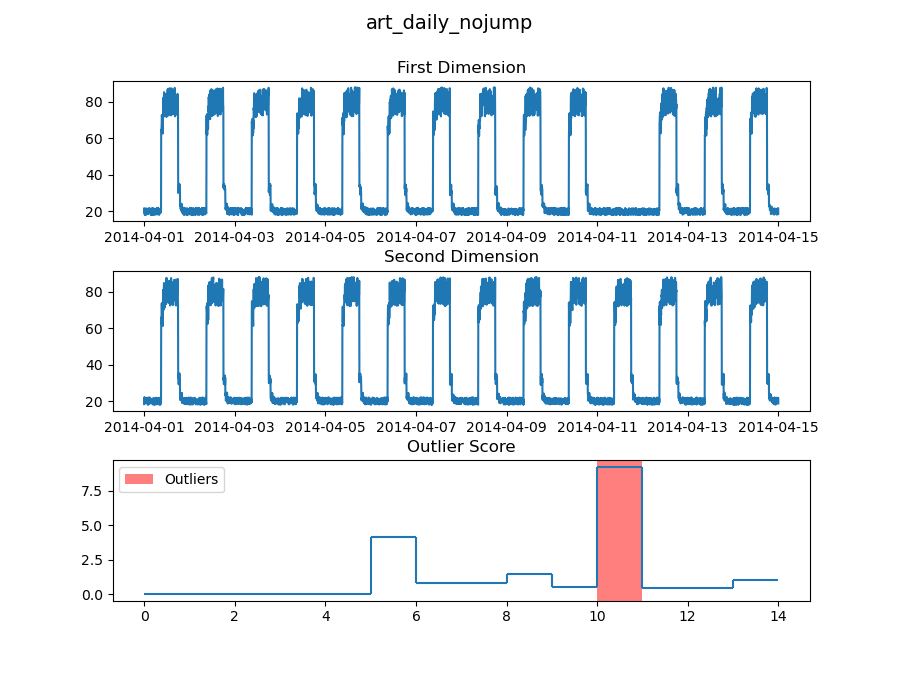
\includegraphics[width=0.5\textwidth]{fig/resultsNetismile/2D/art_daily_nojump}}
	\label{img:isomappictures2}
\end{figure}

\newpage
\subsubsection{Ergebnisse vollst�ndiger Graphen}
\begin{figure}[H]
	\centering
	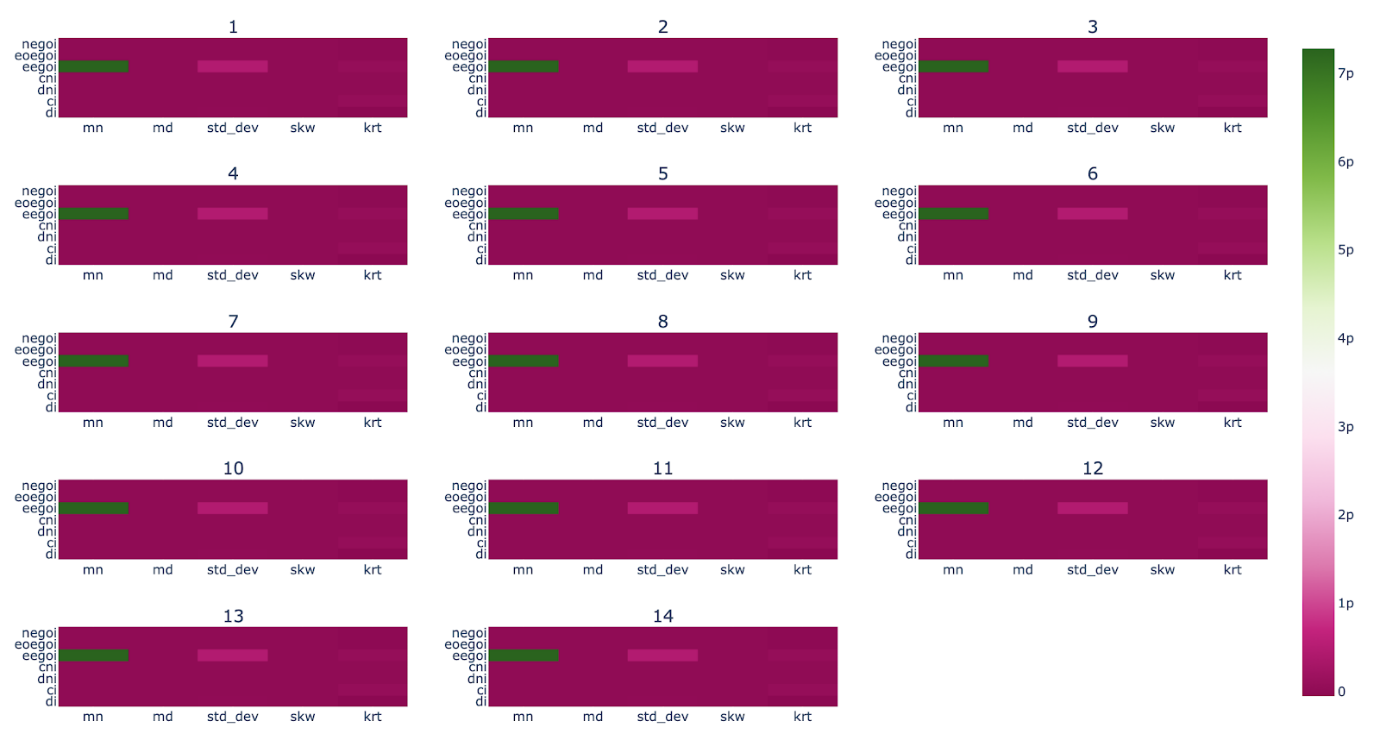
\includegraphics[height=0.8\linewidth,width=\linewidth]{fig/netsimile/heatmap_1}
	\caption{Signaturvektoren der Zeitreihe mit vollst�ndigen Graphen}
	\label{img:netsimile:heatmap_1}
\end{figure}

\begin{figure}[H]
	\centering
	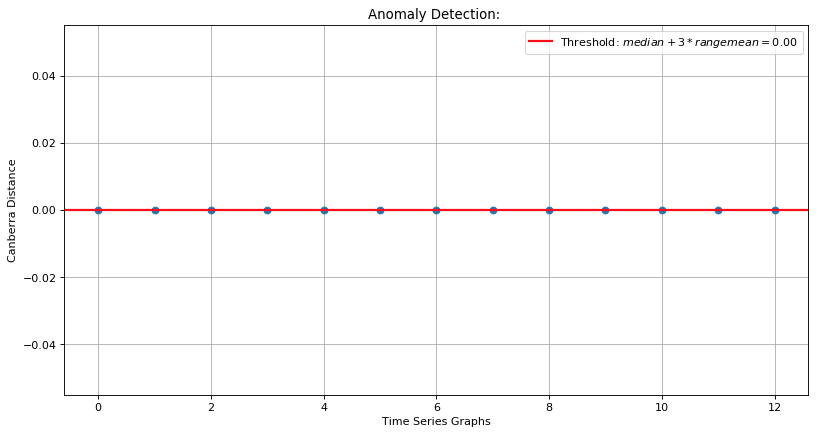
\includegraphics[height=0.6\linewidth,width=\linewidth]{fig/netsimile/anomalie_1}
	\caption{Ausrei�er Score der vollst�ndigen Graphen}
	\label{img:netsimile:anomalie_1}
\end{figure}


\workTodo{Wrong picture for daily peaks. Change that the sixed element is not always an outlier}